% This work is licensed under the Creative Commons Attribution-NonCommercial 4.0 International License.
% To view a copy of this license, visit http://creativecommons.org/licenses/by-nc/4.0/
% or send a letter to Creative Commons, PO Box 1866, Mountain View, CA 94042, USA.

% !TEX TS-program = xelatex

\documentclass[../Main/chem532-notes.tex]{subfiles}

\begin{document}

\chapter[The molecular Hamiltonian]{The molecular Hamiltonian and the Born--Oppenheimer approximation}

\section{Atomic Units}
When we study atoms and molecules, it is convenient to express positions, masses, and other properties in units that are close to one, so we can avoid carrying very large or small powers of 10.
The most common units used in quantum chemistry are \textbf{atomic units} (abbreviated a.u.). Atomic units are defined by the following conditions:
\begin{align}
\text{electron mass} & = m_e = 1\\
\text{electron charge} & = e = 1\\
\text{action} & = \hbar = \frac{h}{2\pi} = 1\\
\text{Coulomb's constant} & = k_e = \frac{1}{4\pi \epsilon_0} = 1
\end{align}
where $\epsilon_0$ is the vacuum permittivity.

The following table reports conversion factors between atomic units and other units 
\begin{table}[htbp]
\centering
\begin{tabular}{lll}
\toprule
Dimension & Symbol (Name) & Value in Other Units\\
\midrule
Length & $a_0$ (bohr) & 0.52918 \AA{} = 0.52918 $10^{-10}$ m\\ 
Mass & $m_e$ & $9.1095 \times 10^{-31}$ Kg \\
Charge & $e$ & $1.6022 \times 10^{-19}$ C \\
Action & $\hbar$ & $1.05457 \times 10^{-34}$ J $\cdot$ s \\
%Coulomb's constant & $\frac{1}{4\pi \epsilon_0}$ & $ \times 10^{-34}$ J $\cdot$ s \\
Energy & $E_{\rm h}$ (Hartree) & 627.51 kcal/mol \\
& & 27.211 eV \\
& & 219474.63 cm$^{-1}$ \\
& & $4.3598 \times 10^{-18}$ J\\
Time & & $2.41889 \times 10^{-17}$ s $\approx 1/41.3$ fs\\
\bottomrule
\end{tabular}
%\caption{Remember, \emph{never} use vertical lines in tables.}
\label{tab:atomicunits}
\end{table}

The speed of light in atomic units is $c = \alpha^{-1}\approx 137$ a.u.\mnote{$\alpha$ is the fine-structure constant $\alpha = \frac{e^2}{4\pi \epsilon_0 \hbar c}$ = 0.007 297 352 562 8(6), which in atomic units reduces to $\alpha = \frac{1}{c}$.}

\newpage

\section{The molecular Hamiltonian}
Consider a molecule containing $N$ electrons and $M$ nuclei.

\begin{center}
\includegraphics[width=2.5in]{../molecular-hamiltonian/coordinates.pdf}
\end{center}

We will start by introducing the notation used to define the molecular Hamiltonian.
The position of the nuclei will be indicated with $\vec{R}_A = \mathbf{R}_A = (x_A,y_A,z_A)$ and that of electrons with $\vec{r}_i = \mathbf{r}_i = (x_i,y_i,z_i)$.
The remaining quantities are summarized in the table below.
\begin{table}[h]
\centering
\begin{tabular}{lcc}
& Nuclei & Electrons \\
\hline
Total number & N & M \\
Index & $A, B, \ldots$ & $i, j, \ldots$ \\
Position & $\vec{R}_A$ & $\vec{r}_i$ \\
Mass & $M_A$ & $1$ \\
Charge & $Z_A$ & $-1$ \\
\end{tabular}
\end{table}

In the absence of external potentials or fields, the total Hamiltonian is given by
\begin{equation}
\hat{H} = \hat{T}_\mathrm{e} +\hat{T}_\mathrm{N} +  \hat{V}_\mathrm{ee} + \hat{V}_\mathrm{eN} + \hat{V}_\mathrm{NN},
\end{equation}
where
\begin{align}
\hat{T}_\mathrm{e} &= -\frac{\hbar^2}{2 m_e} \sum_i^N \nabla^2_i, \\
\hat{T}_\mathrm{N} &= -\frac{\hbar^2}{2} \sum_A^M \frac{1}{M_A} \nabla^2_A, \\
\hat{V}_\mathrm{ee} &= +\sum_{i}^{N}\sum_{j > i}^{N} \frac{1}{4 \pi \epsilon_0} \frac{e^2}{r_{ij}},\\
\hat{V}_\mathrm{eN} &= - \sum_{i}^{N} \sum_{A}^{M} \frac{1}{4 \pi \epsilon_0} \frac{e^2 Z_A}{r_{iA}}, \\
\hat{V}_\mathrm{NN} &= +\sum_{A}^{M} \sum_{B > A}^{M} \frac{1}{4 \pi \epsilon_0} \frac{e^2 Z_A Z_B}{r_{AB}},
\end{align}
and the quantity $r_{ij}$ is the distance between electrons labeled with indices $i$ and $j$
\begin{equation}
r_{ij} = |\vec{r}_i - \vec{r}_j| = \sqrt{(x_i-x_j)^2 + (y_i-y_j)^2 + (z_i-z_j)^2},
\end{equation}
and $r_{iA} = |\vec{r}_i - \vec{R}_A|$ and $r_{AB} = |\vec{R}_A - \vec{R}_B|$ are defined similarly.

In atomic units the Hamiltonian is more compact:
\begin{equation}
\label{eq:molecular_hamiltonian}
\hat{H} =
-\frac{1}{2} \sum_i^N \nabla^2_i
-\frac{1}{2} \sum_A^M \frac{1}{M_A} \nabla^2_A
+ \sum_{i}^{N}\sum_{j > i}^{N} \frac{1}{r_{ij}}
- \sum_{i}^{N} \sum_{A}^{M} \frac{Z_A}{r_{iA}}
+ \sum_{A}^{M} \sum_{B > A}^{M} \frac{Z_A Z_B}{r_{AB}},
\end{equation}
where $M_A$ is understood to be the mass of nucleus $A$ in atomic units.

If we define the collective electronic ($\mathbf{r} = \{ \vec{r}_i \}$) and nuclear ($\mathbf{R} = \{ \vec{R}_A \}$) degrees of freedom, we may write the Schr\"{o}dinger equation compactly as:
\begin{equation}
\hat{H} \Psi_k(\mathbf{r},\mathbf{R}) = E_k \Psi_k(\mathbf{r},\mathbf{R}).
\end{equation}

Note that $\Psi_k(\mathbf{r},\mathbf{R})$ is a complicated function of $3(N+M)$ variables (excluding spin) because it depends both on the coordinate of the electrons and nuclei. For a free molecule it includes translational, rotational, vibrational, and electronic degrees of freedom.
The terms that make this Hamiltonian difficult to solve are those that couple electrons and nuclei, that is, $\hat{V}_\mathrm{NN}$, $\hat{V}_\mathrm{eN}$, and $\hat{V}_\mathrm{eN}$ is problematic because it couples electrons and nuclei.

\begin{problem}	
What does the spectrum of $\hat{H}$ look like for a diatomic molecule?
\end{problem}


\section{Average value of the kinetic and potential energy}

The virial theorem can provide some useful constraints on the properties of stationary states.
%For the Hamiltonian
%\begin{equation}
%\hat{H} = \hat{T} + \hat{V}
%= \sum_i \frac{-1}{2 m_i} \nabla_i^2 + \hat{V}
%\end{equation}
Starting from the condition
\begin{equation}
\frac{d}{dt} \braket{\sum_p \vec{r}_p \hat{\vec{p}}_p} = 0,
\end{equation}
it is possible to show that if the potential $\hat{V} =  \hat{V}_\mathrm{ee} + \hat{V}_\mathrm{eN} + \hat{V}_\mathrm{NN}$ is a homogeneous function of order $k$,\mnote{A homogeneous function of order $k$, $f(\mathbf{x})$ is such that if we scale the argument by $s$ the function is scaled by $s^k$, that is $f(s \mathbf{x}) = s^k f(\mathbf{x})$.} then the expectation value of the kinetic and potential operators are related by
\begin{equation}
2 \braket{\hat{T}} -k \braket{\hat{V}} = 0.
\end{equation}
For Coulombic interactions $k = -1$ and so we have
\begin{equation}
\braket{\hat{V}} = -2 \braket{\hat{T}}.
\end{equation}
And
\begin{equation}
E = \braket{\hat{T}} + \braket{\hat{V}} = - \braket{\hat{T}} = \frac{\braket{\hat{V}}}{2} < 0.
\end{equation}


\section{The Born--Oppenheimer approximation}
One way to simplify the molecular Hamiltonian is to recognize that since electrons and nuclei have very different masses (the smallest value that $M_A$ can have is 1837 $m_e$, for the hydrogen atom) and treat the electronic and nuclear degrees of freedom separately.
More precisely, we are going to assume that we can break down the wave function into a product of an electronic wave function [$\Phi_{\mathrm{el}}(\mathbf{r};\mathbf{R})$] and a nuclear wave function [$\chi_{\mathrm{nuc}}(\mathbf{R})$]
\begin{equation}
\begin{split}
\Psi(\mathbf{r},\mathbf{R}) \approx \Phi_{\mathrm{el}}(\mathbf{r};\mathbf{R}) \chi_{\mathrm{nuc}}(\mathbf{R}).
\end{split}
\end{equation}
Note that the nuclear coordinates $\mathbf{R}$ enter in the electronic wave functions as a parameter, hence we use the symbol ``;'' to separate it from the electron coordinates $\mathbf{r}$. The nuclear wave function is instead independent of the electron coordinates; however, this does not mean that it will be independent from the electronic wave function (see later).

If we plug this trial state in the Schr\"{o}dinger equation, we get the following equation
\begin{equation}
\label{eq:schrodinger_equation_factorized_ansatz}
\begin{split}
(\hat{T}_\mathrm{e} + \hat{T}_\mathrm{N} + \hat{V}_\mathrm{ee} + \hat{V}_\mathrm{eN} +\hat{V}_\mathrm{NN}) \Phi_{\mathrm{el}}(\mathbf{r};\mathbf{R}) \chi_{\mathrm{nuc}}(\mathbf{R})
= E \Phi_{\mathrm{el}}(\mathbf{r};\mathbf{R}) \chi_{\mathrm{nuc}}(\mathbf{R})
\end{split}
\end{equation}
These five operators act on the wave function in different ways.
The kinetic energy operators take derivates with respect to coordinates, while the potential operators just multiply the wave function by a number.
The kinetic energy operator for the electrons acts only on the electronic coordinates and so we can write
\begin{equation}
\hat{T}_\mathrm{e} \Phi_{\mathrm{el}}(\mathbf{r};\mathbf{R}) \chi_{\mathrm{nuc}}(\mathbf{R})
= \chi_{\mathrm{nuc}}(\mathbf{R}) \hat{T}_\mathrm{e} \Phi_{\mathrm{el}}(\mathbf{r};\mathbf{R}).
\end{equation}
The nuclear kinetic energy operator complicates things a bit, because when we apply it to the wave function we get three terms
\begin{equation}
\begin{split}
\hat{T}_\mathrm{N}  \Phi_{\mathrm{el}}(\mathbf{r};\mathbf{R}) \chi_{\mathrm{nuc}}(\mathbf{R})
 = &  -\frac{1}{2} \sum_A^M \frac{1}{M_A} \nabla^2_A \left[  \Phi_{\mathrm{el}}(\mathbf{r};\mathbf{R}) \chi_{\mathrm{nuc}}(\mathbf{R}) \right] \\
= &  -\frac{1}{2} \sum_A^M \frac{1}{M_A}
\chi_{\mathrm{nuc}}(\mathbf{R})  \nabla^2_A  
\Phi_{\mathrm{el}}(\mathbf{r};\mathbf{R}) \\
& 
 - \sum_A^M \frac{1}{M_A}
 \nabla_A\chi_{\mathrm{nuc}}(\mathbf{R})  \cdot \nabla_A  
\Phi_{\mathrm{el}}(\mathbf{r};\mathbf{R}) \\
& 
 -\frac{1}{2} \sum_A^M \frac{1}{M_A}
 \Phi_{\mathrm{el}}(\mathbf{r};\mathbf{R})  \nabla^2_A \chi_{\mathrm{nuc}}(\mathbf{R}).
\end{split}
\end{equation}
The first and second terms on the right hand side of this equation couple the electronic and nuclear degrees of freedom.
If we neglect them and keep only the last term,
\begin{equation}
\begin{split}
\hat{T}_\mathrm{N}  \Phi_{\mathrm{el}}(\mathbf{r};\mathbf{R}) \chi_{\mathrm{nuc}}(\mathbf{R})
\approx 
 -\frac{1}{2} \sum_A^M \frac{1}{M_A}
 \Phi_{\mathrm{el}}(\mathbf{r};\mathbf{R})  \nabla^2_A \chi_{\mathrm{nuc}}(\mathbf{R}).
\end{split}
\end{equation}
 we can rewrite the Schr\"{o}dinger equation as
\begin{equation}
\begin{split}
\Phi_{\mathrm{el}}(\mathbf{r};\mathbf{R})   \hat{T}_\mathrm{N} \chi_{\mathrm{nuc}}(\mathbf{R}) + \chi_{\mathrm{nuc}}(\mathbf{R}) (\hat{T}_\mathrm{e} + \hat{V}_\mathrm{ee} + \hat{V}_\mathrm{eN} +\hat{V}_\mathrm{NN}) \Phi_{\mathrm{el}}(\mathbf{r};\mathbf{R}) 
= E \Phi_{\mathrm{el}}(\mathbf{r};\mathbf{R}) \chi_{\mathrm{nuc}}(\mathbf{R})
\end{split}
\end{equation}
To get this expression we collected all the wave functions not affected by operators to the left side of each term. Next we collect all the terms in the following way
\begin{equation}
\begin{split}
\chi_{\mathrm{nuc}}(\mathbf{R})(\hat{T}_\mathrm{e} + \hat{V}_\mathrm{ee} + \hat{V}_\mathrm{eN} +\hat{V}_\mathrm{NN}) \Phi_{\mathrm{el}}(\mathbf{r};\mathbf{R}) 
=\Phi_{\mathrm{el}}(\mathbf{r};\mathbf{R})    ( E - \hat{ T}_\mathrm{N}) 
\chi_{\mathrm{nuc}}(\mathbf{R})
\end{split},
\end{equation}
and finally divide each side by $\Phi_{\mathrm{el}}(\mathbf{r};\mathbf{R})\chi_{\mathrm{nuc}}(\mathbf{R})$ to get
\begin{equation}
\label{eq:molecular_hamiltonian:bo_derivation}
\begin{split}
\frac{1}{\Phi_{\mathrm{el}}(\mathbf{r};\mathbf{R}) } (\hat{T}_\mathrm{e} + \hat{V}_\mathrm{ee} + \hat{V}_\mathrm{eN} +\hat{V}_\mathrm{NN}) \Phi_{\mathrm{el}}(\mathbf{r};\mathbf{R}) = \frac{1}{\chi_{\mathrm{nuc}}(\mathbf{R})
}  ( E - \hat{ T}_\mathrm{N}) 
\chi_{\mathrm{nuc}}(\mathbf{R})
\end{split}
\end{equation}
The left and right sides of this equation must be equal for any values of $\mathbf{r}$ and $\mathbf{R}$, but since the right side does not depend on $\mathbf{r}$, both sides must depend only the variable $\mathbf{R}$.
Let us call this quantity $V(\mathbf{R})$.
Then Eq.~\eqref{eq:molecular_hamiltonian:bo_derivation} corresponds to two set of conditions
\begin{equation}
\label{eq:molecular_hamiltonian:electronic_se}
(\hat{T}_\mathrm{e} + \hat{V}_\mathrm{ee} + \hat{V}_\mathrm{eN} +\hat{V}_\mathrm{NN} ) \Phi_{\mathrm{el}}(\mathbf{r};\mathbf{R}) = V(\mathbf{R}) \Phi_{\mathrm{el}}(\mathbf{r};\mathbf{R}),
\end{equation}
and
\begin{equation}
\label{eq:molecular_hamiltonian:nuclear_se}
[\hat{ T}_\mathrm{N} + V(\mathbf{R}) ] \chi_{\mathrm{nuc}}(\mathbf{R})  =E \chi_{\mathrm{nuc}}(\mathbf{R}).
\end{equation}

Eqs.~\eqref{eq:molecular_hamiltonian:electronic_se} and \eqref{eq:molecular_hamiltonian:nuclear_se} are coupled equations.
We can find their solution by first solving the Schr\"{o}dinger equation for the electrons assuming that the nuclei are fixed in space ($\mathbf{R}$ is a constant).
Eq.~\eqref{eq:molecular_hamiltonian:electronic_se} is equivalent to the following \textbf{electronic} Schr\"{o}dinger equation
\begin{equation}
\label{eq:molecular_hamiltonian:electronic_se2}
(\hat{H}_\mathrm{el} + \hat{V}_\mathrm{NN})\Phi_{\mathrm{el},k}(\mathbf{r};\mathbf{R})
= V_{k}(\mathbf{R}) \Phi_{\mathrm{el},k}(\mathbf{r};\mathbf{R}).
\end{equation}
where the \textbf{electronic} Hamiltonian ($\hat{H}_{\rm el}$) is defined as:
\begin{equation}
\hat{H}_\mathrm{el} = \hat{T}_\mathrm{e} + \hat{V}_\mathrm{eN} + \hat{V}_\mathrm{ee}.
\end{equation}
Note that there are multiple solutions of the electronic Schr\"{o}dinger equation, so different pairs of eigenvalues/eigenfunctions are labeled by the state index $k$, which can take the values 0, 1, \ldots. The state with $k = 0$  is called the \textbf{ground electronic state}, while states with $k > 0$ are \textbf{excited electronic states}.
The function $V_{k}(\mathbf{R})$ is commonly known as the \textbf{potential energy surface} (abbreviates as PES).
Note that $V_{k}(\mathbf{R})$ gives us the potential energy at a given molecular geometry $\mathbf{R}$ and therefore it describes a set of surfaces in $3M + 1$ dimensions (nuclear coordinates plus energy).

Note that since for a fixed geometry $\hat{V}_\mathrm{NN}$ is a constant (it depends only on the relative positions of the nuclei), we can in practice solve the following eigenvalue problem
\begin{equation}
\label{eq:molecular_hamiltonian:electronic_se3}
\hat{H}_\mathrm{el}\Phi_{\mathrm{el},k}(\mathbf{r};\mathbf{R})
= E_{\mathrm{el}, k}(\mathbf{R}) \Phi_{\mathrm{el},k}(\mathbf{r};\mathbf{R}).
\end{equation}
which has the same eigenfunctions [$\Phi_{\mathrm{el},k}(\mathbf{r};\mathbf{R})$] but different eigenvalues [$E_{\mathrm{el}, k}(\mathbf{R})$].
The quantity $E_{\mathrm{el}, k}(\mathbf{R})$ is also called the \textbf{electronic energy} and it is related to $V_{k}(\mathbf{R})$ via the equation
\begin{equation}
V_{k}(\mathbf{R}) = E_{\mathrm{el},k}(\mathbf{R}) + \sum_{A}^{M} \sum_{B > A}^{M} \frac{Z_A Z_B}{r_{AB}}.
\end{equation}


The concept of the potential energy surface is at the basis of many concepts used to describe molecules like, the molecular geometry, transition states, etc.
The equilibrium geometry of a molecule in a given electronic state $k$, $\mathbf{R}_\mathrm{eq}$, is defined as the minimum of $V_{k}(\mathbf{R})$, that is, the gradient of $V_{k}(\mathbf{R})$ at this geometry is zero
\begin{equation}
\left. \frac{\partial V_{k}(\mathbf{R})}{\partial \mathbf{R}} \right|_{\mathbf{R}= \mathbf{R}_\mathrm{eq}}= 0,
\end{equation}
and the curvature of $V_{k}(\mathbf{R})$ at $\mathbf{R}_\mathrm{eq}$ is positive (the eigenvalues of the second derivative matrix or Hessian are all positive).
Note that for a given electronic state the equilibrium geometry may be unique or there might be several minima with the same energy.
In certain cases, the ground state might not be a bound molecular state (e.g., for dications like \ce{Li_2^{2+}} the energy minimum corresponds to the molecule dissociated into two \ce{Li^{+}} atoms).

\begin{example}[Potential energy surface of H$_2^+$]
The following plot shows the contributions of the electronic energy ($E_\mathrm{el}$) and the nuclear repulsion energy ($V_\mathrm{NN}$) to the potential energy of the ground state of H$_2^+$.
\begin{center}
\includegraphics[width =4.5in]{../molecular-hamiltonian/h2+_pec.pdf}
\end{center}
\end{example}

Although there are $3M$ nuclear degrees of freedom (DOF), in absence of an external potential translations and rotations of a molecule do not change the value of $V_{k}(\mathbf{R})$. Therefore, the number of internal degrees of freedom that change the value of $V_{k}(\mathbf{R})$ is less than $3M$. For a non-linear molecule we have that
\begin{equation}
\text{internal DOF} = \underbrace{3 M}_{\text{total DOF}}
-\underbrace{3}_{\text{rotations}}
-\underbrace{3}_{\text{translations}} = 3M - 6,
\end{equation}
while for a linear molecule
\begin{equation}
\text{internal DOF} = \underbrace{3 M}_{\text{total DOF}}
-\underbrace{2}_{\text{rotations}}
-\underbrace{3}_{\text{translations}} =  3M - 5.
\end{equation}

\begin{example}[Diatomic molecule]
For a diatomic molecule there is $2\cdot3 - 5 = 1$ degrees of freedom. In this case $V_{k}(\mathbf{R})$ may be expressed in terms of the bond distance $R$ as $V_{k}(\mathbf{R})$. In this case we call these quantities \textbf{potential energy curves}.
\end{example}





%\begin{figure}[htbp]
%   \centering
%   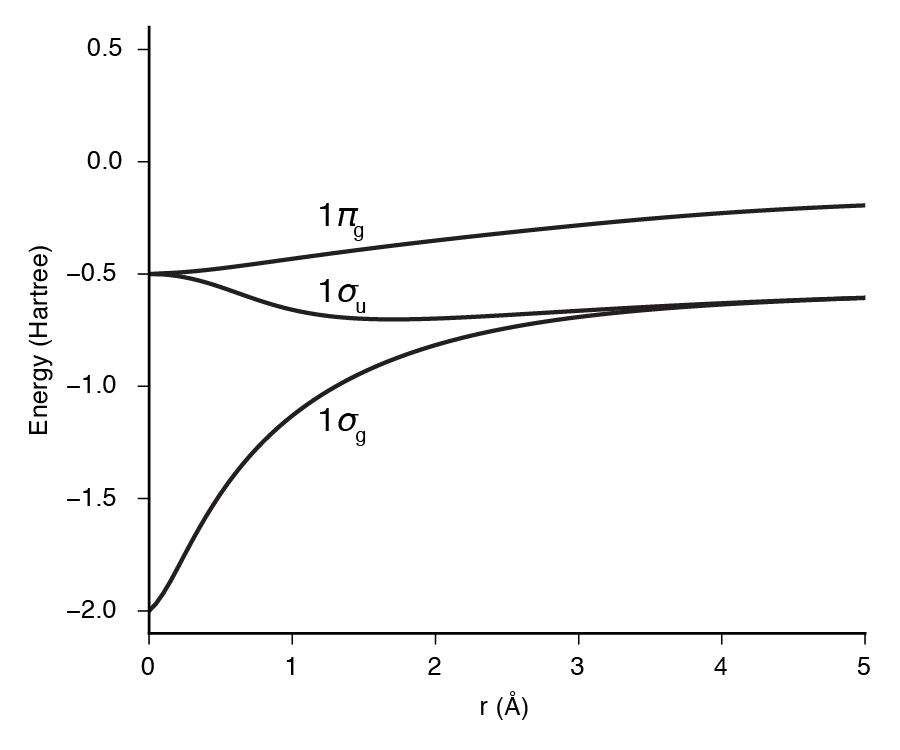
\includegraphics[width=4.5in]{figures/ch2_pec.png}
%   \caption{example caption}
%   \label{fig:example}
%\end{figure}

\section{Avoided crossings}
In this section we discuss some properties of potential energy surfaces. We are particularly interested in understanding when two surfaces become degenerate, because in this case the Born--Oppenheimer approximation is no longer qualitatively correct.
Consider two electronic states $\tilde{\Phi}_1(\mathbf{R})$ and $\tilde{\Phi}_2(\mathbf{R})$ that are not eigenfunctions of the electronic Hamiltonian. When do the potential energy surfaces obtained by diagonalizing the Hamiltonian in this basis become degenerate? 

Let us write the electronic Hamiltonian in the general\mnote{Here we do not assume that $\tilde{\Phi}_1$ and $\tilde{\Phi}_2$ are eigenfunctions of the Hamiltonian.} basis $\{\tilde{\Phi}_1(\mathbf{R}),\tilde{\Phi}_2(\mathbf{R})\}$ omitting the dependence on the coordinate $\mathbf{R}$
\begin{equation}
\mathbf{H}_\mathrm{el} = 
\begin{pmatrix}
\bra{\tilde{\Phi}_1} \hat{H}_\mathrm{el} \ket{\tilde{\Phi}_1} & \bra{\tilde{\Phi}_1} \hat{H}_\mathrm{el} \ket{\tilde{\Phi}_2}\\
\bra{\tilde{\Phi}_2} \hat{H}_\mathrm{el} \ket{\tilde{\Phi}_1} & \bra{\tilde{\Phi}_2} \hat{H}_\mathrm{el} \ket{\tilde{\Phi}_2}
\end{pmatrix}
=
\begin{pmatrix}
\tilde{E}_{1} & V \\
V^* & \tilde{E}_{2}
\end{pmatrix},
\end{equation}
where we used the fact that the Hamiltonian is Hermitian.\mnote{Because the Hamiltonian is Hermitian we have that $\bra{\tilde{\Phi}_2} \hat{H} \ket{\tilde{\Phi}_1} = \bra{\tilde{\Phi}_1} \hat{H} \ket{\tilde{\Phi}_2}^* =  V^*$.}

The difference between the eigenvalues $E_1$ and $E_2$ of $\mathbf{H}_\mathrm{el}$ is
\begin{equation}
E_2 - E_1 = \sqrt{(\tilde{E}_{2}-\tilde{E}_{1})^2 + 4 |V|^2 }.
\end{equation}
From this equation we deduce that for $E_1$ and $E_2$ to be degenerate, the following conditions must be satisfied \textbf{simultaneously}:
\begin{align}
\label{eq:molecular_hamiltonian:conical_intersection1}
\tilde{E}_{1}(\mathbf{R}) &= \tilde{E}_{2}(\mathbf{R}), \\
\label{eq:molecular_hamiltonian:conical_intersection2}
|V(\mathbf{R})| &= 0,
\end{align}
that is, the states that form our basis must be degenerate and there should be no coupling.

In general, these two conditions are independent. So suppose we find a point $\mathbf{R}^*$ for which Eqs.\eqref{eq:molecular_hamiltonian:conical_intersection1}-\eqref{eq:molecular_hamiltonian:conical_intersection2} are satisfied, then we can ask what is the dimensionality of the space in which these two states are degenerate?
If we consider a system with $M$ atoms and assume that $|V|$ is not zero for all molecular geometries,\mnote{In other words, $|V|$ is only \textbf{accidentally zero}.} then the subset of molecular geometries for which two potential energy surfaces intersect has dimension $3M - 6 - 2 = 3M - 8$ for non-linear molecules and $3M - 5 - 2 = 3M - 7$ for linear molecules.
Here we subtract 2 from the number of degrees of freedom to account for the two constraints that must be satisfied for the levels to be degenerate.
This result tells us when a crossing can happen, and if a crossing can happen, it tells us what is the dimension of the space of degenerate electronic energies.

\begin{example}[Diatomic molecules]
For a diatomic molecule degenerate electronic states live in a $3 \cdot 2 - 7 = -1$ dimensional space.
That is, in general two curves do not cross.
However, if for some reason the coupling $|V| = 0$ for all bond lengths then only one of the two constraints applies.
In this case, degenerate electronic states live in a space of dimension $3 \cdot 2 - 6 = 0$, that is, there may be a finite set of points for which $E_2 = E_1$.
Typical examples of situations when $|V| = 0$ include states with different spin or spatial symmetry.  For example, the singlet and triplet states of H$_2$ are allowed to cross.
Crossings may also occur when two electronic states have different number of electrons.
\end{example}

\section{The nuclear Schr\"{o}dinger equation}
Given the eigenvalues and eigenfunctions of the electronic Hamiltonian, it is possible to obtain wave functions for the nuclei by solving the nuclear Schr\"{o}dinger equation:
\begin{equation}
\hat{H}_{{\rm nuc},k} \chi_{v,k}(\mathbf{R}) =  E_{v,k} \chi_{v,k}(\mathbf{R}),
\end{equation}
where $\hat{H}_{{\rm nuc},k}$ is the nuclear Hamiltonian for electronic state $k$:
\begin{equation}
\hat{H}_{{\rm nuc},k} = \hat{T}_{N} + V_{k}(\mathbf{R}).
\end{equation}
In this approximation, the nuclei experience a potential generated by the electrons plus the nuclear-nuclear repulsion:
\begin{equation}
V_{k}(\mathbf{R}) = \int d\mathbf{r} \; \Phi^*_{\mathrm{el},k} (\mathbf{r};\mathbf{R}) \hat{H}_\mathrm{el}(\mathbf{R}) \Phi_{\mathrm{el},k} (\mathbf{r};\mathbf{R}) + V_\mathrm{NN}(\mathbf{R}).
\end{equation}
This expression is an equivalent way to rewrite $V_{k}(\mathbf{R}) $, and it emphasizes the fact that the potential energy surface is the potential experienced by the nuclei after averaging the interaction with the electrons in the state $\Phi_{\mathrm{el},k} (\mathbf{r};\mathbf{R})$.

Note that the solutions of the nuclear Schr\"{o}dinger equation are \textbf{vibrational levels} of the electronic state $k$.
Since each electronic state has a different shape, the vibrational levels for two electronic states are, in general, different.
In this picture, the electrons react instantaneously to the motion of the nuclei, so the nuclei always see the electrons in a fully relaxed state (adiabatic approximation).
The BO approximation is thus valid when nuclear and electronic motion occur on different time (energy) scales. In practice, the BO approximation is accurate when electronic states are well separated from one another, and, conversely, it fails when two or more electronic states become near-degenerate.
The first corrections to the BO approximation enter at order $\lambda^6 = \left( \frac{m_e}{M} \right)^{3/2}$, which for the hydrogen atom are of the order of $1.3 \cdot 10^{-5}$ \Eh.

\begin{details}	
In deriving the nuclear Schr\"{o}dinger equation we have neglected two terms that arise from the kinetic energy operator for the nuclei. So what happens if we introduce these terms back but still assume the BO factorized wave function for the electrons + nuclei?
Let us go back to the Schr\"{o}dinger equation for the electrons and nuclei where we plugged in the factorized form of the wave function [see Eq.~\eqref{eq:schrodinger_equation_factorized_ansatz}] and left project with the state $\Phi_{\mathrm{el}}^*(\mathbf{r};\mathbf{R})$ and integrate over $\mathbf{r}$ (we momentarily omit the electronic state index $k$ in the next few equations). This gives us
\begin{equation}
\begin{split}
\bra{\Phi_{\mathrm{el}}(\mathbf{r};\mathbf{R})} (\hat{T}_\mathrm{e} + \hat{T}_\mathrm{N}   + \hat{V}_\mathrm{ee} + \hat{V}_\mathrm{eN} +\hat{V}_\mathrm{NN} ) \ket{\Phi_{\mathrm{el}}(\mathbf{r};\mathbf{R})}  \chi_{\mathrm{nuc}}(\mathbf{R})
= E \chi_{\mathrm{nuc}}(\mathbf{R}).
\end{split}
\end{equation}
Using the fact that $(\hat{T}_\mathrm{e} + \hat{V}_\mathrm{eN} + \hat{V}_\mathrm{ee} + \hat{V}_\mathrm{NN} ) \Phi_{\mathrm{el}}(\mathbf{r};\mathbf{R}) = V(\mathbf{R}) \Phi_{\mathrm{el}}(\mathbf{r};\mathbf{R})$, we can simplify this equation to
\begin{equation}
\label{eq:molecular_hamiltonian:diagonal_bo}
\begin{split}
\bra{\Phi_{\mathrm{el}}(\mathbf{r};\mathbf{R})} (\hat{T}_\mathrm{N} +V(\mathbf{R}) ) \ket{\Phi_{\mathrm{el}}(\mathbf{r};\mathbf{R})}  \chi_{\mathrm{nuc}}(\mathbf{R})
= E \chi_{\mathrm{nuc}}(\mathbf{R}).
\end{split}
\end{equation}
The left-hand-side of this equation can be written as the sum of three terms:
\begin{equation}
\begin{split}
& [\hat{T}_\mathrm{N} +V(\mathbf{R})]  \chi_{\mathrm{nuc}}(\mathbf{R})  \\
& 
-\frac{1}{2} \sum_A^M \frac{1}{M_A}
\underbrace{\braket{\Phi_{\mathrm{el}}(\mathbf{r};\mathbf{R})|\nabla_A \Phi_{\mathrm{el}}(\mathbf{r};\mathbf{R})}}_{\text{First-order derivative coupling}}  \cdot \nabla_A \chi_{\mathrm{nuc}}(\mathbf{R}) \\
& 
-\frac{1}{2} \chi_{\mathrm{nuc}}(\mathbf{R}) \sum_A^M \frac{1}{M_A} \underbrace{\braket{\Phi_{\mathrm{el}}(\mathbf{r};\mathbf{R}) |\nabla^2_A \Phi_{\mathrm{el}}(\mathbf{r};\mathbf{R})} }_{\text{Second-order derivative coupling}}  .
\end{split}
\end{equation}
The first term appears in the nuclear Schr\"{o}dinger equation that we have seen before, but the terms in the second and third lines are new.
These are the so-called \textbf{diagonal corrections to the BO approximation} since they involve derivative couplings between the same electronic state.
These terms can be included in the nuclear Schr\"{o}dinger equation [Eq.~\eqref{eq:molecular_hamiltonian:diagonal_bo}] to estimate corrections to the BO approximation.
For heavy nuclei these corrections are somewhat small and so are typically neglected. 
However, diagonal corrections are sometime included in highly-accurate computations.

To go beyond diagonal BO corrections one has to consider solutions to the molecular Hamiltonian that mix various electronic states.
Since at each value of $\mathbf{R}$ the eigenfunctions of the electronic Hamiltonian form a complete basis for the electrons, we can expand the full wave function (electrons plus nuclei) as
\begin{equation}
\label{eq:molecular_hamiltonian:mol_ham_fullci}
\begin{split}
\Psi(\mathbf{r},\mathbf{R}) = \sum_{k=0}^\infty \Phi_{\mathrm{el},k}(\mathbf{r};\mathbf{R}) \chi_{\mathrm{nuc},k}(\mathbf{R}).
\end{split}
\end{equation}
When this equation is substituted in the Schr\"{o}dinger equation it leads to a set of coupled Schr\"{o}dinger  equations that determine the nuclear wave functions $\chi_{\mathrm{nuc},k}(\mathbf{R})$.
Note, however, that these nuclear wave functions are different from the ones we have encountered before.

Eq.~\eqref{eq:molecular_hamiltonian:mol_ham_fullci}  is the most general solution that we can write for a wave function of electrons and nuclei, and it is required when the assumptions made in the Born--Oppenheimer approximation are not valid.
A large number of interesting and important phenomena are associated with the break down of the adiabatic assumption and require a significantly more refined treatment than the one discussed here.
\end{details}
We will come back to the nuclear Schr\"{o}dinger equation after learning how to compute potential energy surfaces.
%

\section*{Study Questions}
\begin{myenumerate}
\item What are atomic units?
\item What is the unit of energy in atomic units?
\item What are the five terms in the molecular Hamiltonian?
\item What how many dimensions does the wave function for the molecular Hamiltonian have?
\item What is the basis for the Born--Oppenheimer approximation?
\item What terms in the expression $\hat{T}_\mathrm{N}  \Phi_{\mathrm{el}}(\mathbf{r};\mathbf{R})$ are neglected when deriving the Born--Oppenheimer approximation?
\item What is the electronic Schr\"{o}dinger equation?
\item What is the electronic Hamiltonian and what operators enter it?
\item What is the difference between the potential energy surface and the electronic energy?
\item Why do Eqs.~\eqref{eq:molecular_hamiltonian:electronic_se2} and \eqref{eq:molecular_hamiltonian:electronic_se3} share the same eigenfunction?
\item How many internal degrees of freedom are there for a linear and a nonlinear molecule?
\item Can two electronic state of the same symmetry cross in a diatomic molecule? What happens if the have the same symmetry?
\item What is the nuclear Schr\"{o}dinger equation?
\item Why do the solutions of the nuclear Schr\"{o}dinger equation depend on the electronic state?
\item What are the diagonal corrections to the BO approximation?
\end{myenumerate}

\end{document}